\documentclass[12pt,a4paper]{article}
\usepackage{lmodern}

\usepackage{placeins}
\usepackage{amssymb,amsmath}
\usepackage{ifxetex,ifluatex}
\usepackage{fixltx2e} % provides \textsubscript
\ifnum 0\ifxetex 1\fi\ifluatex 1\fi=0 % if pdftex
  \usepackage[T1]{fontenc}
  \usepackage[utf8]{inputenc}
\else % if luatex or xelatex
  \ifxetex
    \usepackage{mathspec}
    \usepackage{xltxtra,xunicode}
  \else
    \usepackage{fontspec}
  \fi
  \defaultfontfeatures{Mapping=tex-text,Scale=MatchLowercase}
  \newcommand{\euro}{€}
\fi
% use upquote if available, for straight quotes in verbatim environments
\IfFileExists{upquote.sty}{\usepackage{upquote}}{}
% use microtype if available
\IfFileExists{microtype.sty}{%
\usepackage{microtype}
\UseMicrotypeSet[protrusion]{basicmath} % disable protrusion for tt fonts
}{}
\usepackage[lmargin = 2cm, rmargin = 2.5cm, tmargin = 2cm, bmargin =
2.5cm]{geometry}


% Figure Placement:
\usepackage{float}
\let\origfigure\figure
\let\endorigfigure\endfigure
\renewenvironment{figure}[1][2] {
    \expandafter\origfigure\expandafter[H]
} {
    \endorigfigure
}

%%%% Jens %%%%
\usepackage[tiny]{titlesec}
\DeclareMathOperator*{\argmax}{arg\,max}
\DeclareMathOperator*{\argmin}{arg\,min}
\renewcommand{\vec}{\operatorname{vec}}
\newcommand{\tr}{\operatorname{tr}}
\newcommand{\Var}{\operatorname{Var}} % Variance
\newcommand{\VAR}{\operatorname{VAR}} % Vector autoregression
\newcommand{\Lag}{\operatorname{L}} % Lag operator
\newcommand{\Cov}{\operatorname{Cov}}
\newcommand{\diag}{\operatorname{diag}}
\newcommand{\adj}{\operatorname{adj}}
\newcommand{\loglik}{\operatorname{ll}}

\allowdisplaybreaks

\titleformat{\section}
{\normalfont\large\bfseries}{\thesection}{1em}{}

%### sections
\newcommand{\tmpsection}[1]{}
\let\tmpsection=\section
%\renewcommand{\section}[1]{\tmpsection{\underline{#1}} }
\titleformat*{\section}{\large\bfseries}
\titleformat*{\subsection}{\normalsize\bfseries\sffamily}
%\setkomafont{subsection}{\Large}
%\setkomafont{subsubsection}{\large}
%\setkomafont{paragraph}{\large}
%\setkomafont{subparagraph}{\large}





%% citation setup
\usepackage{csquotes}

\usepackage[backend=biber, maxbibnames = 99, style = apa]{biblatex}
\setlength\bibitemsep{1.5\itemsep}
\addbibresource{R_packages.bib}
\usepackage{graphicx}
\usepackage{subcaption}
\makeatletter
\def\maxwidth{\ifdim\Gin@nat@width>\linewidth\linewidth\else\Gin@nat@width\fi}
\def\maxheight{\ifdim\Gin@nat@height>\textheight\textheight\else\Gin@nat@height\fi}
\makeatother
% Scale images if necessary, so that they will not overflow the page
% margins by default, and it is still possible to overwrite the defaults
% using explicit options in \includegraphics[width, height, ...]{}
\setkeys{Gin}{width=\maxwidth,height=\maxheight,keepaspectratio}
\ifxetex
  \usepackage[setpagesize=false, % page size defined by xetex
              unicode=false, % unicode breaks when used with xetex
              xetex]{hyperref}
\else
  \usepackage[unicode=true, linktocpage = TRUE]{hyperref}
\fi
\hypersetup{breaklinks=true,
            bookmarks=true,
            pdfauthor={Martin Arnold},
            pdftitle={Installation von  und },
            colorlinks=true,
            citecolor=blue,
            urlcolor=blue,
            linkcolor=blue,
            pdfborder={0 0 0}}
\urlstyle{same}  % don't use monospace font for urls
\setlength{\parindent}{0pt}
\setlength{\parskip}{6pt plus 2pt minus 1pt}
\setlength{\emergencystretch}{3em}  % prevent overfull lines
\setcounter{secnumdepth}{5}

%%% Use protect on footnotes to avoid problems with footnotes in titles
\let\rmarkdownfootnote\footnote%
\def\footnote{\protect\rmarkdownfootnote}

%%% Change title format to be more compact
\usepackage{titling}

% Create subtitle command for use in maketitle
\newcommand{\subtitle}[1]{
  \posttitle{
    \begin{center}\large#1\end{center}
    }
}

\setlength{\droptitle}{-2em}
  \title{Installation von \texttt{R} und \texttt{RStudio}}
  \pretitle{\vspace{\droptitle}\centering\huge}
  \posttitle{\par}
\subtitle{R Propädeutikum}
  \author{Martin Arnold}
  \preauthor{\centering\large\emph}
  \postauthor{\par}
  \date{}
  \predate{}\postdate{}


%% linespread settings

\usepackage{setspace}

\onehalfspacing


% Language Setup

\usepackage{ifthen}
\usepackage{iflang}
\usepackage[super]{nth}
\usepackage[ngerman, english]{babel}

%Acronyms
\usepackage[printonlyused, withpage, nohyperlinks]{acronym}
\usepackage{changepage}

% Multicols for the Title page
\usepackage{multicol}


% foot


\begin{document}

\ifthenelse{\equal{german}{german}}{
  \selectlanguage{ngerman}
  }{
  \selectlanguage{english}
  }

%%%%%%%%%%%%%% Jens %%%%%
\numberwithin{equation}{section}
\restoregeometry


%%% Header 

\begin{minipage}{0.6\textwidth}
Universität Duisburg-Essen\\
Fakultät für Wirtschaftswissenschaften\\
Lehrstuhl für Ökonometrie\\
\end{minipage}

%\begin{minipage}{0.4\textwidth}
	\begin{flushright}
	\vspace{-3cm}
	\includegraphics*[width=5cm]{Includes/duelogo_en.png}\\
	\vspace{.125cm}
	\end{flushright}
%\end{minipage}
%\vspace{.125cm}
\hspace{-0.005cm}Wintersemester 2020/2021

\vspace{0.05cm}

\begin{center}
	\vspace{.25cm}
	Martin Arnold \hspace{.5cm} Jens Klenke \\
	\vspace{.25cm}
	\textbf{\Large{Installation von \texttt{R} und \texttt{RStudio}}}\\
	\vspace{.25cm}
	\textbf{\large{R Propädeutikum}}\\
	\vspace{.125cm}
\end{center}




% body from markdown

\hypertarget{installation-unter-windows-1087}{%
\section{Installation unter Windows
10/8/7}\label{installation-unter-windows-1087}}

\hypertarget{r}{%
\subsection{R}\label{r}}

\begin{enumerate}
  \item Laden Sie den \texttt{R}-installer von der \href{https://cran.r-project.org/bin/windows/base/}{\texttt{R}-Projekt Seite} herunter, indem Sie auf die Schaltfläche \textit{Download} (siehe Abbildung \ref{fig:r_side}) klicken.
  \FloatBarrier
    \begin{figure}[h]
        \centering                      
        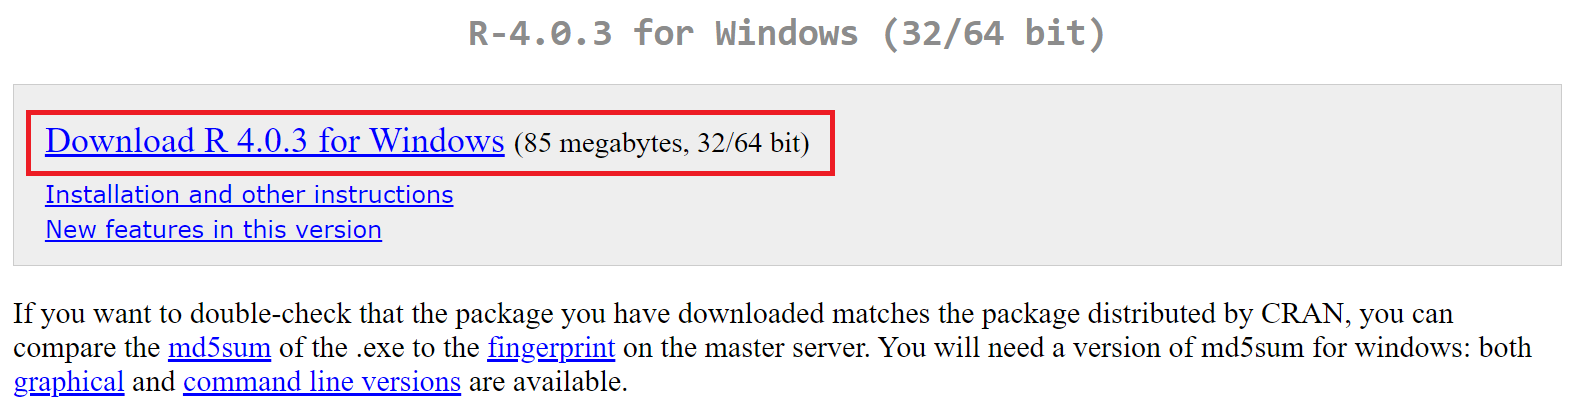
\includegraphics[width=0.8\textwidth]{images/r_projekt_side.PNG}
        \caption{R-Projektseite}
    \label{fig:r_side}
    \end{figure}
    \FloatBarrier
    \item Nach dem Download öffnen Sie den Installer per Doppelklick. Starten Sie anschließend die Installation, indem Sie auf \textit{Ausführen} klicken. 
    \begin{figure}
\centering
\begin{subfigure}{.5\textwidth}
  \centering
  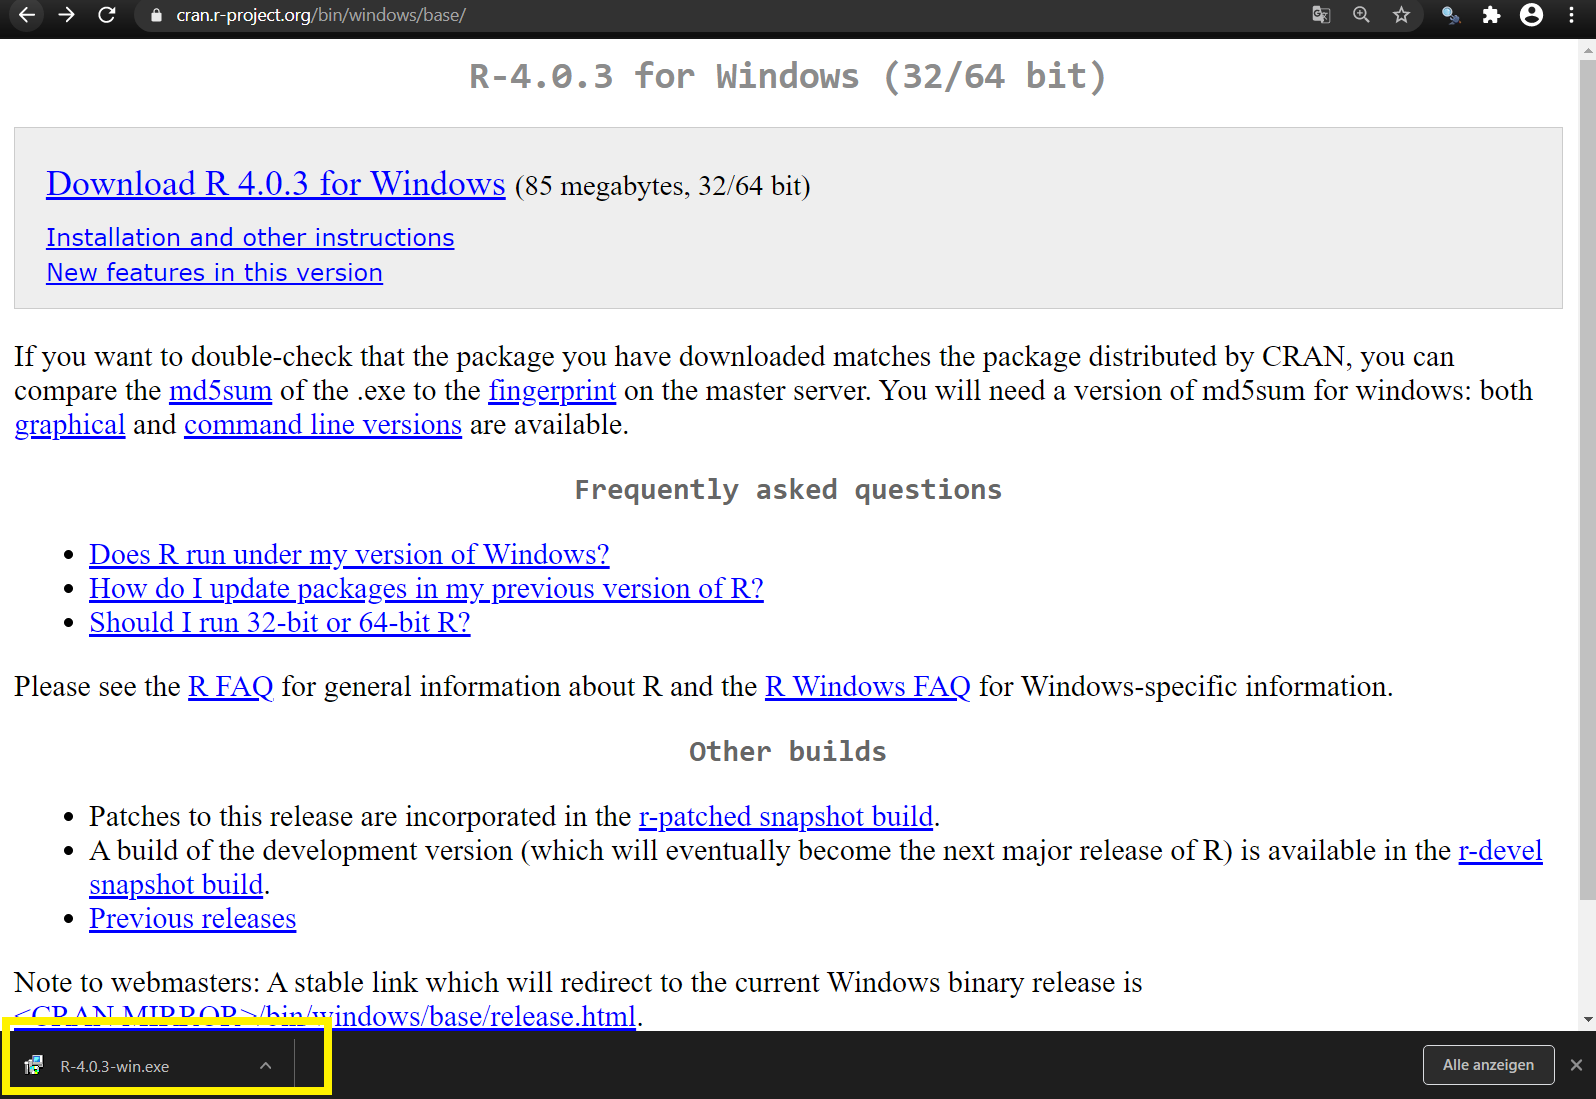
\includegraphics[width=.95\linewidth]{images/overview.PNG}
  \label{fig:sub1}
\end{subfigure}%
\begin{subfigure}{.5\textwidth}
  \centering
  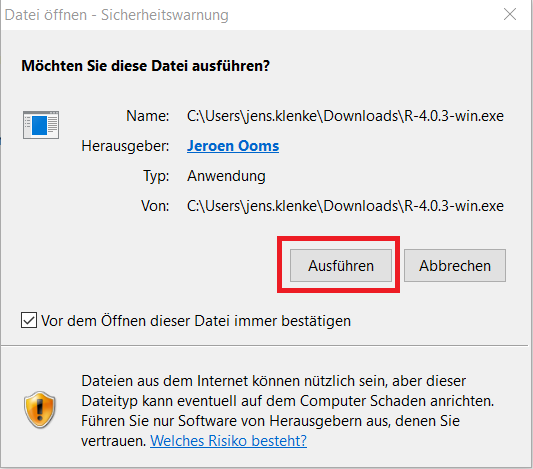
\includegraphics[width=.95\linewidth]{images/ausfuehren.PNG}
  \label{fig:sub2}
\end{subfigure}
\label{fig_start}
\caption{Öffnen der Datei (links), Starten der Installation (rechts)}
\end{figure}
  \item Nachdem Sie die Installationssprache ausgewählt haben, klicken Sie wiederholt auf \textit{Weiter}\footnote{R wird auf diesem Weg mit den Standardeinstellungen installiert.} bis die Schaltfläche \textit{Fertigstellen} erscheint. Klicken Sie dann erneut auf die Schaltfläche. 
  \item Ihre \texttt{R}-Distribution ist nun installiert. 
\end{enumerate}

\hypertarget{rstudio}{%
\subsection{RStudio}\label{rstudio}}

\begin{enumerate}
  \item Der nächste Schritt ist, \texttt{RStudio} von der RStudio-Website \href{https://rstudio.com/products/rstudio/download/#download}{herunterzuladen}.
\FloatBarrier
    \begin{figure}[h]
        \centering                      
        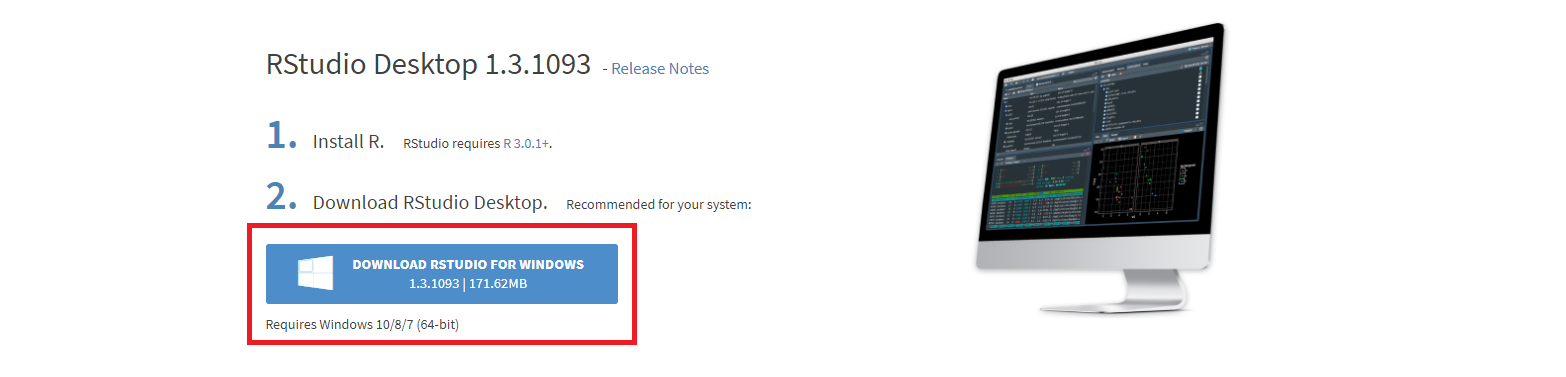
\includegraphics[width=0.95\textwidth]{images/Rstudio.PNG}
        \caption{Download von RStudio}
    \label{fig:rstudio_side}
    \end{figure}
\FloatBarrier
  \item Gehen sie erneut vor wie in Schritt 2 und 3. Ihre \texttt{R-Studio}-Version ist nun installiert. Die Verbindung zu \texttt{R} wird automatisch erstellt.
\end{enumerate}

\hypertarget{installation-unter-macos-x}{%
\section{Installation unter MacOS X}\label{installation-unter-macos-x}}

\hypertarget{r-1}{%
\subsection{R}\label{r-1}}

\begin{enumerate}
  \item Laden Sie den \texttt{R}-installer von der \href{https://cran.r-project.org/bin/macosx/base/}{\texttt{R}-Projekt-Website} herunter, indem Sie auf die Schaltfläche \textit{Download} klicken.
  \FloatBarrier
    \begin{figure}[h]
        \centering                      
        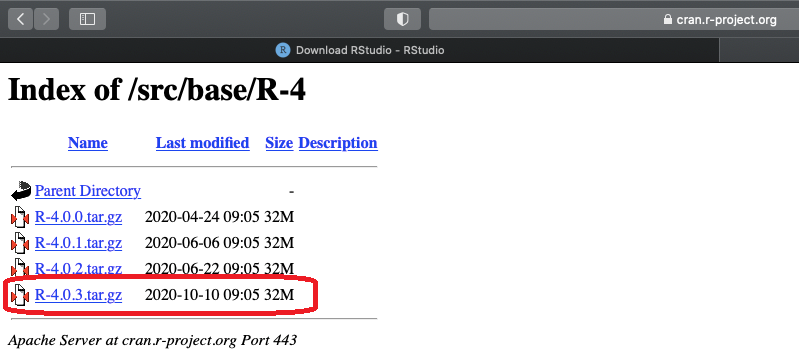
\includegraphics[width=0.8\textwidth]{images/mac_r_seite.PNG}
        \caption{R-Projektseite für MacOS}
    \label{fig:r_side_mac}
    \end{figure}
    \FloatBarrier
    \item Öffnen Sie die .pkg-Datei und führen Sie die Installation durch, indem Sie stets die Schaltfläche \textit{Continue} klicken, bis Sie zum Menüpunkt \textbf{Installation type} gelangen. Starten Sie die Installation mit einem Klick auf \textit{install}.
  \item Ihre \texttt{R}-Distribution ist nun installiert. Schließen Sie den Installer.
\end{enumerate}

\hypertarget{rstudio-1}{%
\subsection{RStudio}\label{rstudio-1}}

\begin{enumerate}
  \item Der nächste Schritt ist, \texttt{RStudio} von der RStudio-Website \href{https://rstudio.com/products/rstudio/download/#download}{herunterzuladen}.
  \item Öffnen Sie die Datei und kopieren Sie die App \texttt{RStudio} in den Ordner Applications, in dem Sie die Datei auf den Ordner ziehen.
  \begin{figure}
\centering
\begin{subfigure}{.5\textwidth}
  \centering
  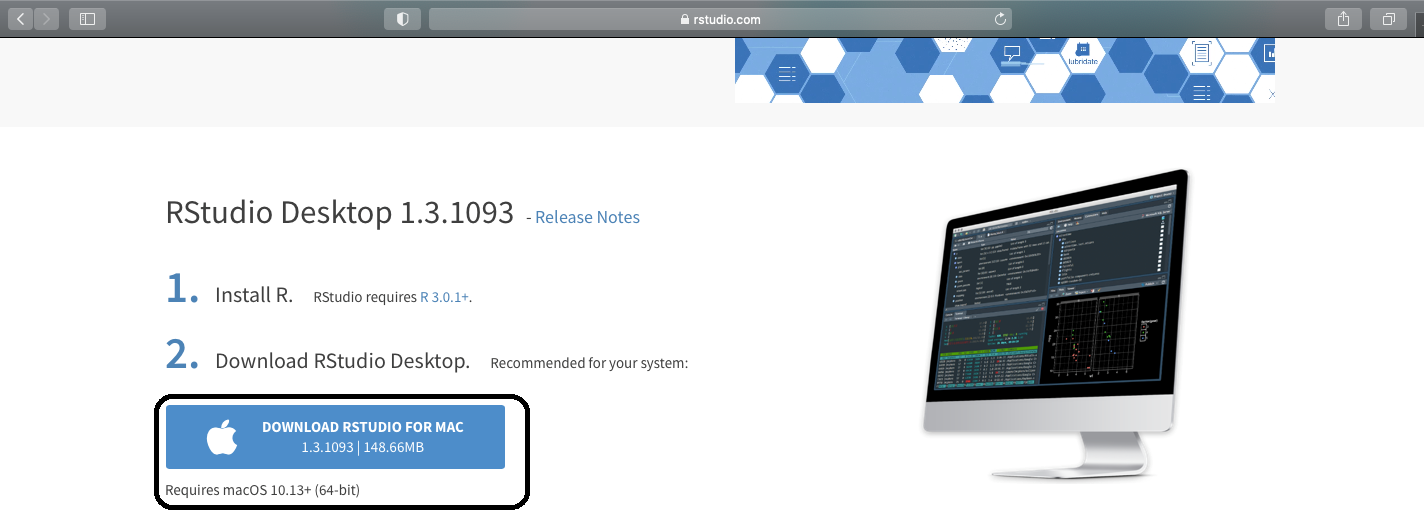
\includegraphics[width=.95\linewidth]{images/r_studio_mac.PNG}
  \label{fig:c}
\end{subfigure}%
\begin{subfigure}{.5\textwidth}
  \centering
  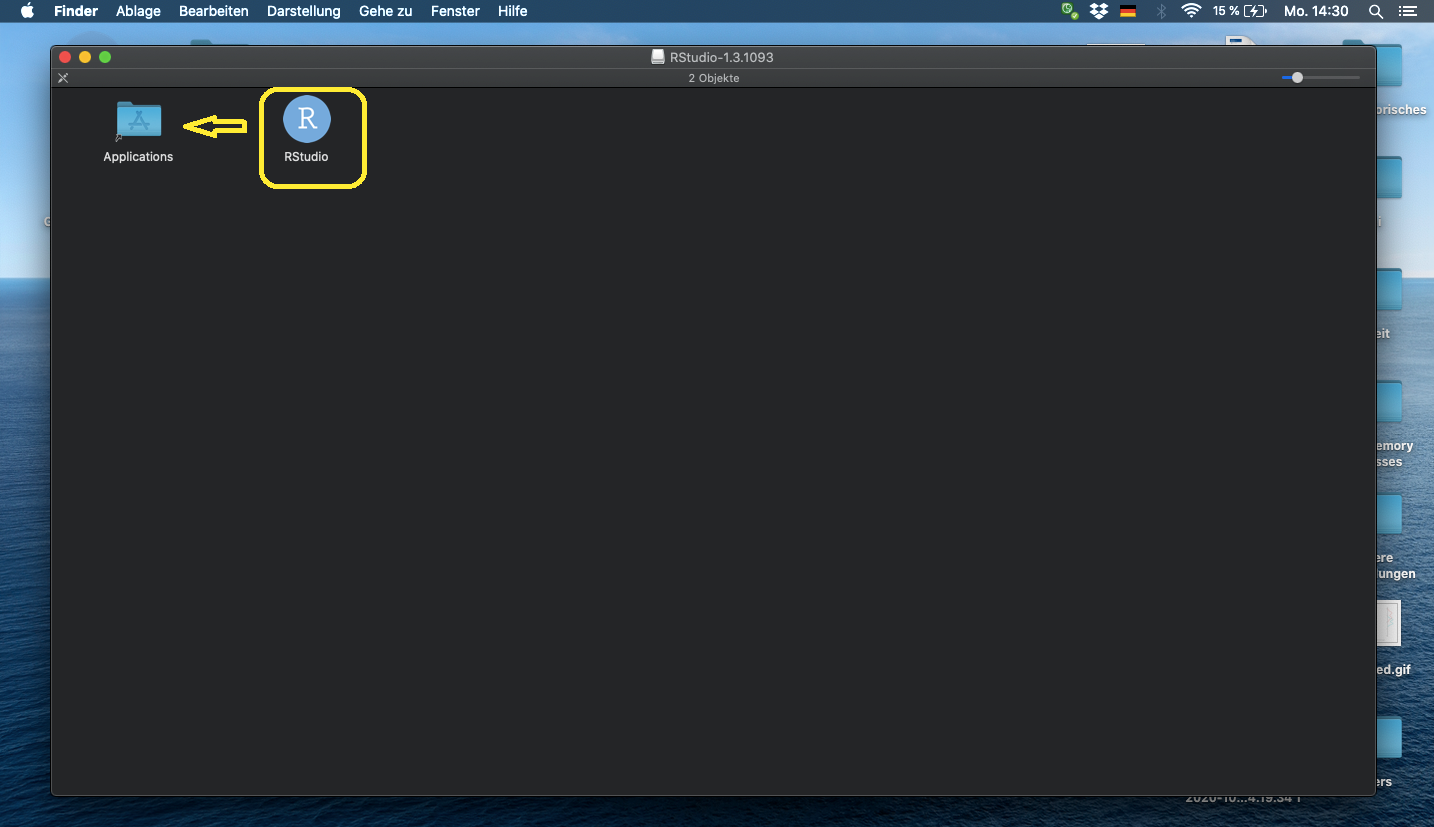
\includegraphics[width=.95\linewidth]{images/mac_r_studio_install.PNG}
  \label{fig:start.mac_sub_2}
\end{subfigure}
\label{fig:start.mac_sub_2}
\caption{Homepage von RStudio (links), Installation von RStudio (rechts)}
\end{figure}
  \item RStudio ist nun installiert. RStudio erkennt die installierte R-Version automatisch.
\end{enumerate}

\end{document}
